
\section{Organisation}

\begin{frame}
  {Kontakt und Sprechstunde}
  \begin{itemize}
    \item Sprechstunde: dienstags 12:15--13:15\\
      \alert{Bitte unbedingt 24h vorher eintragen!}
    \item Büro: JK 31/236 (Rostlaube)
    \item Email: \texttt{roland.schaefer@fu-berlin.de}
      \vspace{\baselineskip}
    \item Klausur: Dienstag, den 18. Februar 2020, 14–16 c.t. in HS 1a und 1b\\
      \rot{Die Klausur für Grundschuldidaktiker*innen findet im Sommer statt!}
      \vspace{\baselineskip}
    \item \alert{Alle Fragen zur Organisation der Klausur richten Sie bitte\\
      an die Dozent*innen der Basisseminare.}
      \vspace{\baselineskip}
    \item \rot{Wichtig: \url{http://rolandschaefer.net/?page_id=1972}}
  \end{itemize}
\end{frame}


\begin{frame}
  {Ablauf und Inhalte der Vorlesung}
  \begin{itemize}
    \item 13 Sitzungen über Grammatik des Deutschen und Linguistik
    \item drei Sitzungen: Anwendung auf Textebene, Übungen für die Klausur 
      \vspace{\baselineskip}
    \item Meine Inhalte entsprechen meiner \alert{\textit{Einführung in\\
      die grammatische Beschreibung des Deutschen:}}\\
      \rot{\textit{Dritte, überarbeitete und erweiterte Auflage}}
    \item \url{http://langsci-press.org/catalog/book/224} (\alert{open access})
      \vspace{\baselineskip}
    \item Bei Amazon für 20€: \url{https://www.amazon.de/dp/3961101183/}
  \end{itemize}
\end{frame}

\begin{frame}
  {Fragen und Interaktion}
  \begin{itemize}
    \item Interaktion in einer VL mit 900 Teilnehmer*innen ist ausgeschlossen.
      \vspace{\baselineskip}
    \item Wenn Sie Fragen zum Stoff oder zum Buch haben:
      \texttt{roland.schaefer@fu-berlin.de}
    \item Ich würde geeignete Fragen auch gerne in meinem Blog beantworten:\\
      \url{http://grammatick.de}
      \vspace{\baselineskip}
    \item \rot{Bitte beachten Sie folgende Hinweise zur Email-Kommunikation:\\
        \url{http://rolandschaefer.net/?page_id=1736}}
  \end{itemize}
\end{frame}

\begin{frame}
  {Der Plan für heute}
  \pause
  \begin{itemize}
    \item Grammatik
      \begin{itemize}
        \item Grammatik als System
        \item Kern und Peripherie des Systems
        \item Norm und Beschreibung, Regel und Regularität
      \end{itemize}
      \vspace{\baselineskip}
      \pause
    \item Grammatik in Schule und Studium
      \begin{itemize}
        \item Bildungssprache
        \item Sprachbetrachtung
        \item Welche Grammatik für das Germanistikstudium?
      \end{itemize}
      \vspace{\baselineskip}
      \pause
    \item EGBD3: Kapitel 1 bis 3
      \pause
    \item \alert{Sie müssen irgendwann vor der Klausur diese Kapitel durcharbeiten.}
  \end{itemize}
\end{frame}


\section{Grammatik}

\begin{frame}
  {Deutsche Sätze erkennen und interpretieren}
  \pause
  \begin{exe}
    \ex Dies ist ein Satz.
  \pause
    \ex Satz dies ein ist.
  \pause
    \ex Kno kna knu.
  \pause
    \ex This is a sentence.
  \pause
    \vspace{\baselineskip}
    \ex Dies ist ein Satz
  \end{exe}
\end{frame}


\begin{frame}
  {Form und Bedeutung: Kompositionalität}
  \begin{exe}
    \ex Das ist ein Kneck.
    \pause
    \vspace{\baselineskip}
  \ex Jede Farbe ist ein Kurzwellenradio.
  \ex Der dichte Tank leckt.
\end{exe}
    \vspace{\baselineskip}
  \pause

  \Large\begin{block}{Kompositionalität}
    Die Bedeutung komplexer sprachlicher Ausdrücke ergibt sich aus der Bedeutung ihrer Teile und der Art ihrer grammatischen Kombination. 
    Diese Eigenschaft von Sprache nennt man Kompositionalität.
  \end{block}
\end{frame}

\begin{frame}
  {Grammatik als System und Grammatikalität}
  \pause

  \Large\begin{block}{Grammatik}
    Eine Grammatik ist ein \alert{System von Regularitäten}, nach denen aus einfachen Einheiten komplexe Einheiten einer Sprache gebildet werden.
  \end{block}
  \vspace{\baselineskip}

  \pause

  \begin{block}{Grammatikalität}
    Jede von einer bestimmten Grammatik beschriebene Symbolfolge ist \alert{grammatisch} relativ zu dieser Grammatik, alle anderen sind \alert{ungrammatisch}.
  \end{block}
\end{frame}

\begin{frame}
  {(Un)grammatisch ist nicht gleich (in)akzeptabel}
  \pause
  \begin{exe}
    \ex\begin{xlist}
      \ex Bäume wachsen werden hier so schnell nicht wieder.
      \pause
      \ex Touristen übernachten sollen dort schon im nächsten Sommer.
      \pause
      \ex Schweine sterben müssen hier nicht.
      \pause
      \ex Der letzte Zug vorbeigekommen ist hier 1957.
      \pause
      \ex Das Telefon geklingelt hat hier schon lange nicht mehr.
      \pause
      \ex Häuser gestanden haben hier schon immer.
      \pause
      \ex Ein Abstiegskandidat gewinnen konnte hier noch kein einziges Mal.
      \pause
      \ex Ein Außenseiter gewonnen hat hier erst letzte Woche.
      \pause
      \ex Die Heimmannschaft zu gewinnen scheint dort fast jedes Mal.
      \pause
      \ex Ein Außenseiter gewonnen zu haben scheint hier noch nie.
      \pause
      \ex Ein Außenseiter zu gewinnen versucht hat dort schon oft.
      \pause
      \ex Einige Außenseiter gewonnen haben dort schon im Laufe der Jahre.
    \end{xlist}
  \end{exe}
\end{frame}

\begin{frame}
  {Kern und Peripherie}
  \pause
\begin{exe}
  \ex\label{ex:kernundperipherie022}
    \begin{xlist}
      \ex \alert{Baum, Haus, Matte, Döner, Angst, Öl, Kutsche, \ldots}
      \ex \rot{System, Kapuze, Bovist, Schlamassel, Marmelade, Melodie, \ldots}
    \end{xlist}
    \pause
    \ex
    \begin{xlist}
      \ex \alert{geht, läuft, lacht, schwimmt, liest, \ldots}
      \ex \rot{kann, muss, will, darf, soll, mag}
    \end{xlist}
    \pause
    \ex
    \begin{xlist}
      \ex \alert{des Hundes, des Geistes, des Tisches, des Fußes, \ldots}
      \ex \rot{des Schweden, des Bären, des Prokuristen, des Phantasten, \ldots}
    \end{xlist}
  \end{exe}
  \pause
  \vspace{\baselineskip}
  \Large
  \centering
  \alert{Hohe Typenhäufigkeit} vs.\ \rot{niedrige Typenhäufigkeit}.  
\end{frame}

\begin{frame}
  {Zwei verschiedene Häufigkeiten}
  \pause
  \Large\begin{block}{Typenhäufigkeit}
    Wie viele \alert{verschiedene} Realisierungen (=~Typen)\\
    einer Sorte linguistischer Einheiten gibt es?
  \end{block}

  \pause
  \vspace{\baselineskip}
  
  \begin{block}{Tokenhäufigkeit}
    Wie häufig sind die \alert{ggf.\ identischen} Realisierungen\\
    (=~Tokens) einer Sorte linguistischer Einheiten?
  \end{block}
\end{frame}

\begin{frame}
  {Beispiel: Modalverben als Peripherie}
  \pause
  \centering 
    \begin{tabular}{lrr}
    \lsptoprule
    \multirow{2}{*}{\textbf{Modalverb}} & \textbf{Anteil an} & \textbf{eine Form pro}\\
    & \textbf{allen Wortformen} & \textbf{Textwörter (Mittel)}\\
    \midrule
    \textit{können} & 0,53\% &   189 \\
    \textit{müssen} & 0,21\% &   476 \\
    \textit{sollen} & 0,19\% &   526 \\
    \textit{wollen} & 0,13\% &   769 \\
    \textit{mögen}  & 0,06\% & 1.666\\
    \textit{dürfen} & 0,05\% & 2.000\\
    \lspbottomrule
  \end{tabular}\\
  \vspace{\baselineskip}
  \footnotesize Die Zahlen basieren auf DECOW16A \citep{SchaeferBildhauer2012}, Tabelle aus \citet[11]{Schaefer2018}.
\end{frame}

\begin{frame}
  {Regel vs.\ Regularität bzw.\ Generalisierung}
  \pause
  \begin{exe}
    \ex
    \begin{xlist}
      \ex{Relativsätze und eingebettete \textit{w}-Sätze werden nicht\\
    durch Komplementierer eingeleitet.}
      \pause
      \ex{\textit{fragen} ist ein schwaches Verb.}
      \pause
      \ex{\textit{zurückschrecken} bildet das Perfekt mit dem Hilfsverb \textit{sein}.}
      \pause
      \ex{Im Aussagesatz steht vor dem finiten Verb genau ein Satzglied.}
      \pause
      \ex{In Kausalsätzen mit \textit{weil} steht das finite Verb an letzter Stelle.}
    \end{xlist}
  \end{exe}
\end{frame}


\begin{frame}
  {Normkorm? Regularitätenkonform?}
  \pause
  \begin{exe}
    \ex
    \begin{xlist}
      \ex Dann sieht man auf der ersten Seite \alert{wann, wo und wer} \rot{dass} kommt.
      \pause
      \ex Er \rot{frägt} nach der Uhrzeit.
      \pause
      \ex Man \rot{habe} zu jener Zeit nicht vor Morden \alert{zurückgeschreckt}.
      \pause
      \ex \rot{Der Universität} \alert{zum Jubiläum} gratulierte auch Bundesminister Dorothee Wilms, die in den fünfziger Jahren in Köln studiert hatte.
      \pause
      \ex Das ist Rindenmulch, \alert{weil} hier \rot{kommt} noch ein Weg.
    \end{xlist}
  \end{exe}
\end{frame}


\begin{frame}
  {Regel und Regularität}
  \pause
  \begin{block}{Regularität}
    Eine grammatische Regularität innerhalb eines Sprachsystems liegt dann vor, wenn sich Klassen von Symbolen unter vergleichbaren Bedingungen gleich (und damit vorhersagbar) verhalten.
  \end{block}

  \pause
  \vspace{0.5\baselineskip}

  \begin{block}{Regel}
    Eine grammatische Regel ist die Beschreibung einer Regularität, die in einem normativen Kontext geäußert wird.
  \end{block}

  \pause
  \vspace{0.5\baselineskip}
  
  \begin{block}{Generalisierung}
    Eine grammatische Generalisierung ist eine durch Beobachtung zustandegekommene Beschreibung einer Regularität.
  \end{block}
\end{frame}

\begin{frame}
  {Norm ist Beschreibung}
  \pause
  \begin{itemize}[<+->]
    \item Norm als Grundkonsens
    \item Sprache und Norm im Wandel
    \item Norm und Situation (Register, Stil, \dots)
    \item Variation in der Norm
      \vspace{\baselineskip}
    \item \alert{Wichtigkeit der Norm, insbesondere im schulischen Deutschunterricht}
  \end{itemize}
\end{frame}

\section{Grammatik im Lehramtsstudium}

\begin{frame}
  {Bildungssprache in der siebten Jahrgangsstufe}
  \pause
  Aufgabe: In eigenen Worten die Aufgabe wiedergeben\\
  (\citealt{GogolinLange2011}; s.\ \citealt{Feilke2012}).\\[0.5\baselineskip]
  \pause
  \centering
  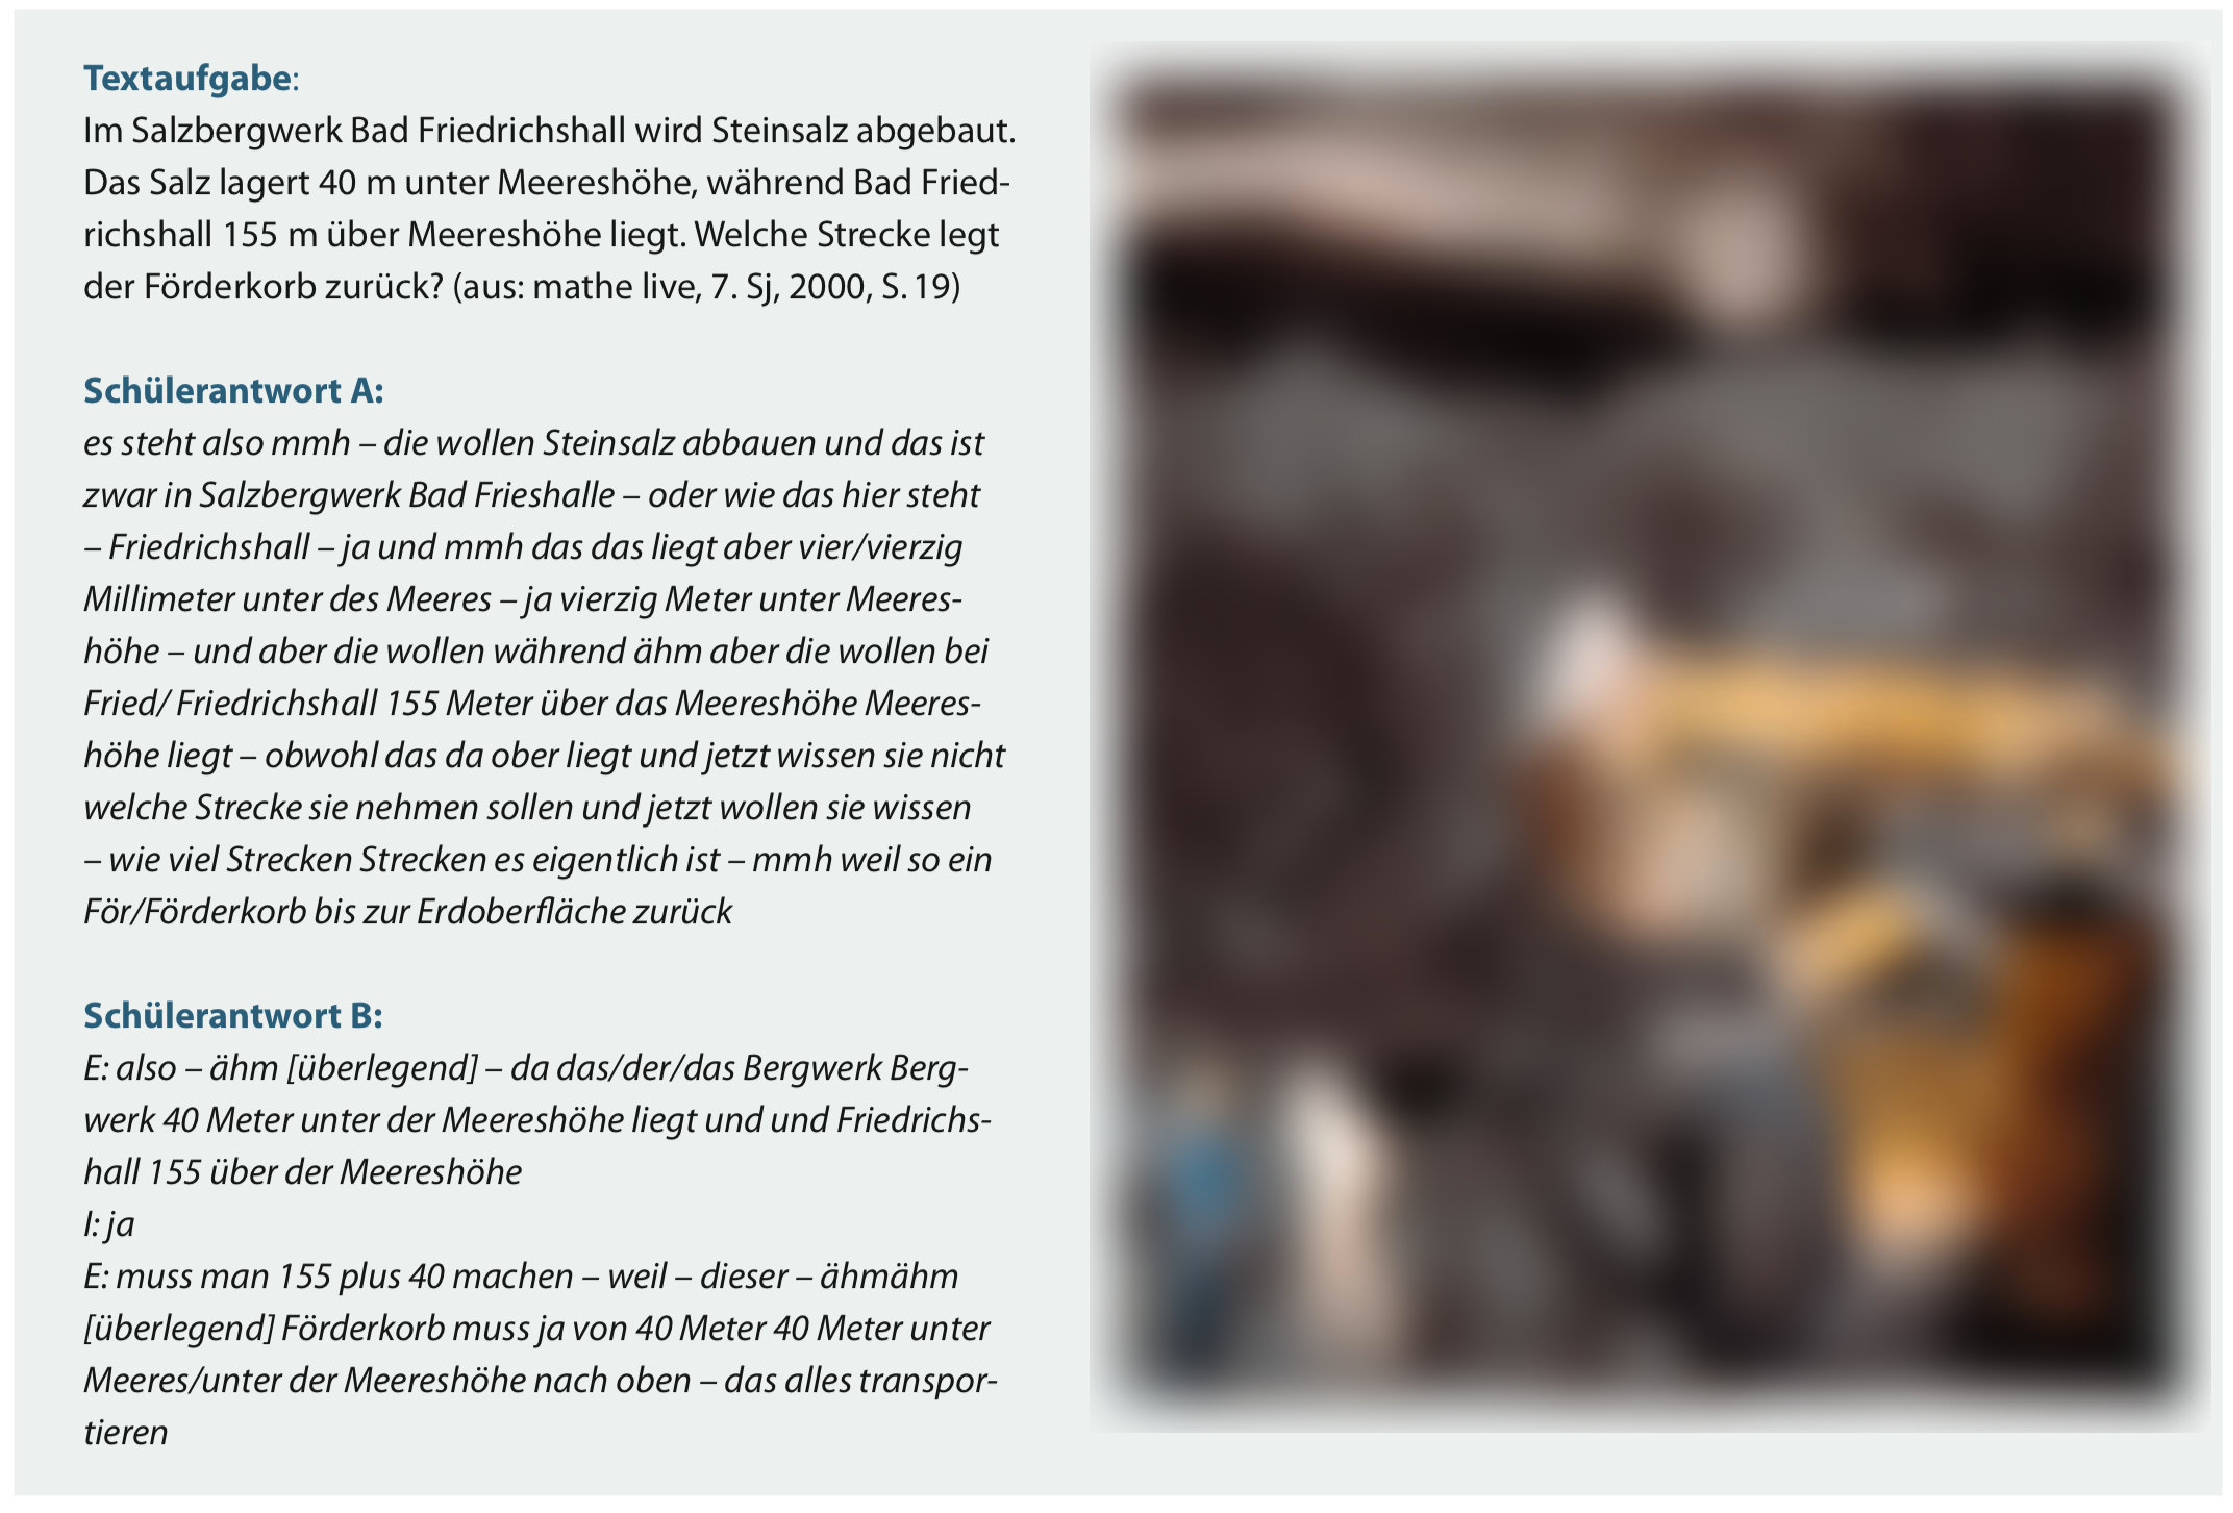
\includegraphics[height=0.68\textheight]{graphics/feilke_blur}
\end{frame}

\begin{frame}
  {Sprachbetrachtung und Literatur im Deutsch-Abitur I}
  \pause
  Sprachlich-grammatische Betrachtung zur Literatur in Abiturarbeiten\\
  \citep{Haecker2009}.\\[\baselineskip]
  \pause
  \centering
  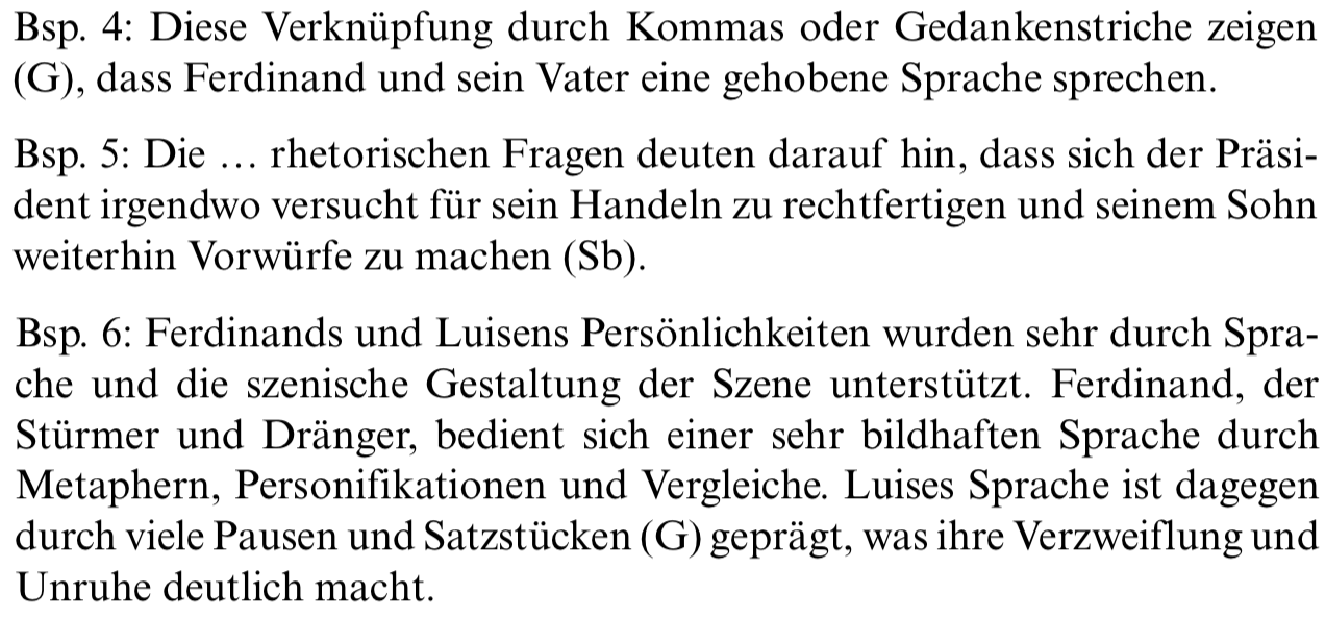
\includegraphics[height=0.5\textheight]{graphics/haecker1}
\end{frame}

\begin{frame}
  {Sprachbetrachtung und Literatur im Deutsch-Abitur II}
  Sprachlich-grammatische Betrachtung zur Literatur in Abiturarbeiten\\
  \citep{Haecker2009}.\\[\baselineskip]
  \centering
  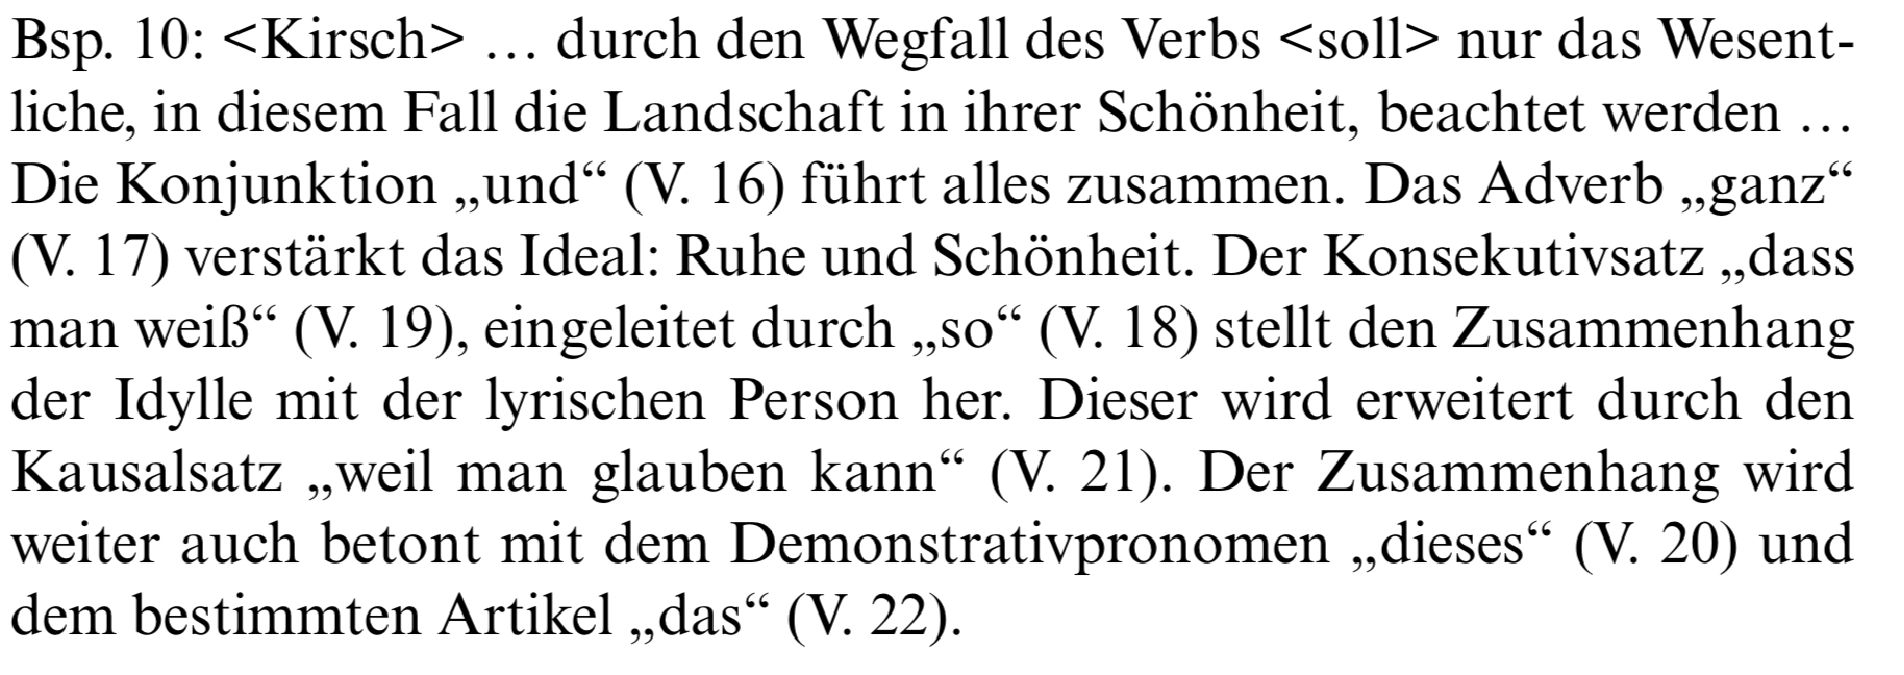
\includegraphics[height=0.4\textheight]{graphics/haecker2}
\end{frame}

\begin{frame}
  {Bildungssprache}
  \pause
  \alert{\textit{Der Deutschunterricht führt zu einem kompletten Umbau\\
  der Grammatik des Kindes.}} (nach \citealt{Bredel2013,Eisenberg2004})\\[\baselineskip]
  \pause
  \begin{itemize}[<+->]
    \item Anforderungen:
    \begin{itemize}[<+->]
      \item Darstellung komplexer Sachverhalte
      \item \dots und nicht-faktischer (z.\,B.\ hypothetischer) Sachverhalte
      \item Intensionalität
      \item Registerbewusstsein
    \end{itemize}
        \vspace{\baselineskip}
      \item Eigenschaften:
    \begin{itemize}[<+->]
      \item dekontextualisiert
      \item schriftorientiert
      \item normorientiert
    \end{itemize}
        \vspace{\baselineskip}
      \item \alert{Das alles ist verknüpft mit spezifischen grammatischen Formen!}
  \end{itemize}
\end{frame}

\begin{frame}
  {Sprachbetrachtung}
  \pause
  \begin{itemize}[<+->]
    \item Bildungssprache $\Leftrightarrow$ Sprachbetrachtung
      \vspace{\baselineskip}
    \item Bewusstsein über richtige und angemessene Form
      \vspace{\baselineskip}
    \item explizite Sprachbetrachtung im Alltag:
      \begin{itemize}[<+->]
        \item Selbst- oder Fremdkorrektur
        \item Suche nach dem richtigen Ausdruck
        \item Orthographie optimieren
        \item Texte optimieren
        \item Begriffe definieren
        \item Grammatikalität beurteilen
      \end{itemize}
  \end{itemize}
\end{frame}

\begin{frame}
  {Ausgangsbasis: vorliterate Kinder und Sprachbetrachtung}
  \pause
  Klassische Studien nach \citet{Bredel2013}, s.\,a.\ \citet[57--58]{Schaefer2018}:\\
  \vspace{\baselineskip}
  \pause
  \begin{itemize}[<+->]
    \item \alert{bedeutungsbezogene} bzw.\ \alert{holistische} Betrachtung
    \item \textit{Welches Wort ist länger: Haus oder Streichholzschächtelchen?} --- \textit{Haus.}
    \item Assoziationen zu Substantiven wie \textit{Bett}: \alert{Ereignisse} \textit{schlafen gehen} usw.\\
      Erwachsene: \alert{Substantive} für andere Möbel usw.
    \item \textit{Warum heißt der Geburtstag  "`Geburtstag"'?} ---\\
      \textit{"`Weil es Geschenke und Kuchen gibt."'}
    \item \textit{Wieviele Wörter in "`Im alten Haus lebt eine junge Frau."'} --- \textit{Zwei.}
    \item \textit{Wieviele Wörter in "`Alex hat sieben Schwestern."'} --- \textit{Sieben.}
      \vspace{\baselineskip}
    \item Aber \alert{erfolgreich}: \textit{Benenne das letzte Wort des Satzes.}
    \item[$\Rightarrow$] Die mentale Grammatik basiert auf Wörtern,\\
      der sprachbetrachtende Zugriff allerdings noch nicht.
  \end{itemize}
\end{frame}

\begin{frame}
  {Schulunterricht}
  \begin{itemize}[<+->]
    \item \alert{systematisch}
      \begin{itemize}
        \item in knapper Zeit das Ganze im Blick
      \end{itemize}
      \vspace{\baselineskip}
    \item funktional im Sinn von \alert{Form-Funktion-Beziehung}
      \begin{itemize}
        \item Formen systematisieren
        \item erst dann auf Funktionen beziehen
      \end{itemize}
      \vspace{\baselineskip}
    \item \alert{induktiv}
      \begin{itemize}
        \item keine rein deduktive Anwendung vorgegebener Begriffe
        \item Erkenntnisprozesse über sprachliche Formen und Funktionen
        \item \alert{\textit{Grammatik machen}} (Eisenberg)
      \end{itemize}
  \end{itemize}
\end{frame}

\begin{frame}
  {Aufgaben von Lehrpersonen}
  \pause
  \alert{\textit{Lehrkräften wird die Sprache der Lernenden anvertraut.}} \citep{Eisenberg2004}\\[\baselineskip]
  \pause
  \begin{itemize}[<+->]
    \item Unterrichten der Schrift, Orthographie und Schreibung
    \item Unterweisung in Bildungssprache\slash Sprachbetrachtung
    \item Erkennen und \alert{Einordnen} von \alert{sprachlichen Defiziten}
    \item Erkennen von \alert{Interferenz mit Dialekt bzw.\ anderen Erstsprachen}
    \item \alert{Bewerten} von sprachlichen Leistungen
    \item \alert{Erklären} der Bewertung (auch gegenüber Eltern)
      \vspace{\baselineskip}
    \item[$\Rightarrow$] Anforderung: vertieftes Wissen über Sprache, vor allem Grammatik
    \item[$\Rightarrow$] Methode der sprachlichen Analyse über Faktenwissen hinaus
    \item[$\Rightarrow$] \rot{Die Grammatik für Studierende des Lehramts ist eine völlig andere\\
      als die, die sie später an Schulkinder und Jugendliche vermitteln!}
  \end{itemize}
\end{frame}


\begin{frame}
  {Wie war das?}
  Ich wiederhole zur Sicherheit nochmal\ldots\\
  \vspace{\baselineskip}
  \pause
  \begin{center}
    \Large\rot{Die Grammatik für Studierende des Lehramts\\
    ist eine völlig andere als die, die sie später \\
    an Schulkinder und Jugendliche vermitteln!}
  \end{center}
\end{frame}

\begin{frame}
  {"`Wozu brauchen wir das denn?"'}
  \pause
  \begin{itemize}[<+->]
    \item Diese Frage gilt hiermit als nachhaltig beantwortet.
    \item Linguistik und Fachdidaktik: keine praktische Anleitungen\\
      für erfolgreiche Schulstundenkonzepte
    \item Grundausbildung im \alert{Umgang mit Sprache} (Linguistik)\\
      und zum \alert{richtigen Handeln im Unterricht} (Fachdidaktik)
      \vspace{\baselineskip}
    \item Minimalforderung: \alert{Examinierte Lehrkräfte müssen\\
      die Aufgaben für die späteren Lernenden selber lösen und\\
      in den Gesamtkontext einordnen können.}
    \item \alert{Bis nächste Woche: Bitte schauen Sie sich den Fragebogen\\
      aus Schäfer \& Sayatz (2017) an (siehe Blackboard und Webseite).}
  \end{itemize}
\end{frame}

\section{Vorschau}

\begin{frame}
  {Phonetik: die Beschreibung der Aussprache}

  \begin{itemize}[<+->]
    \item Besprechung des Fragebogens sowie \citet{SchaeferSayatz2017a}
      \Zeile
    \item Medien der Sprachübermittlung
    \item Wie bilden wir Sprachlaute?
    \item Wo bilden wir Sprachlaute?
    \item deutsche Standardaussprache (Bundesrepublik)
    \item genaue Transkription von Sprachlauten
      \Zeile
    \item \rot{Lesen Sie bitte: Kapitel 4 \textit{Phonetik}}
  \end{itemize}

  \pause
  \pause
  \pause
  \pause
  \pause
\end{frame}
